\documentclass[tikz,border=5pt]{standalone}

\usepackage{libertinus}
%\usepackage{libertinusmath}
\usepackage{tikz}

\begin{document}

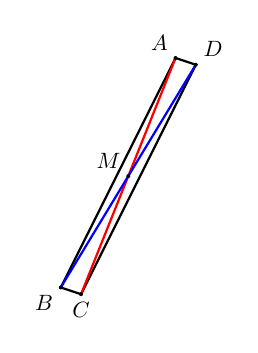
\begin{tikzpicture}[scale=0.6, every node/.style={scale=0.8}]

% Points
\coordinate (A) at (1,3);
\coordinate (B) at (-10/7,-13/7);
\coordinate (C) at (-1,-2);
\coordinate (D) at (10/7,20/7);

% Parallelogram
\draw[thick] (A)--(B)--(C)--(D)--cycle;

% Diagonals
\draw[red, thick] (A)--(C);
\draw[blue, thick] (B)--(D);

% Midpoint
\coordinate (M) at (0,0.5);

% Points
\fill (A) circle (1.2pt) node[above left] {$A$};
\fill (B) circle (1.2pt) node[below left] {$B$};
\fill (C) circle (1.2pt) node[below] {$C$};
\fill (D) circle (1.2pt) node[above right] {$D$};
\fill (M) circle (1.2pt) node[above left] {$M$};

\end{tikzpicture}

\end{document}
